\documentclass[11pt,b5paper,papersize,dvipdfmx]{jsarticle}

\usepackage{amsmath,amssymb,cases} %数学関係
\usepackage[dvipdfmx]{graphicx} %図の挿入
\usepackage{wrapfig} %文章中に図
\usepackage{here} %Hで図を強制出力
\usepackage{physics}
\usepackage[svgnames]{xcolor} % tikzより前に読み込む必要あり
\usepackage{tikz} % おえかきできるお



\begin{document} % ----------------------


\section{tikz}

\begin{figure}[H]
  \centering
  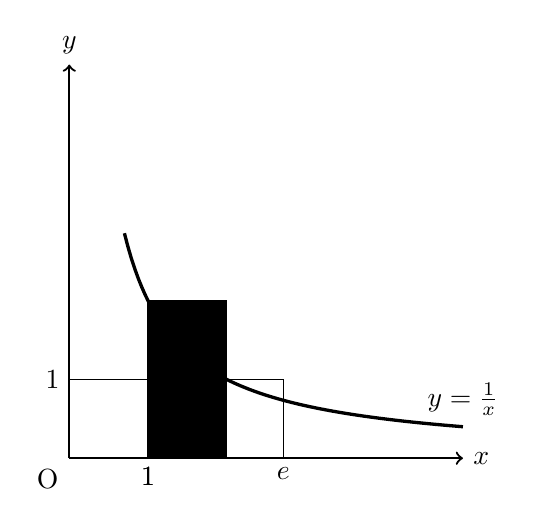
\begin{tikzpicture}[domain=0:5, samples=100, very thick] % 定義域、点の数、線幅
    \draw (0,0) node[below left]{O}; % 原点、0でも、above, below, left, rightで位置指定
    % 位置指定はanchor=north, south, east, westでも可能
    \draw[thick, ->] (0,0)--(5,0) node[right] {$x$}; % x軸、[->]で矢印、他に[-stealth]等
    \draw[thick, ->] (0,0)--(0,5) node[above] {$y$}; % y軸
    \draw [domain=0.7:5] plot(\x, 2/\x) node[above] {$y=\frac1x$};
    \draw [thin](0,1) node [left]{$1$}--(e,1)--(e,0) node[below]{$e$}; % 補助線
    \draw [thin](1,0) node [below]{$1$}--(1,1);
    \draw [thin](1,0) node [below]{$1$}--(1,2)--(2,2)--(2,0);
    \fill (1,0)--(1,2)--(2,2)--(2,0);
  \end{tikzpicture}
  \label{fig:tikz-2}
  \caption{tikzの例2}
\end{figure}

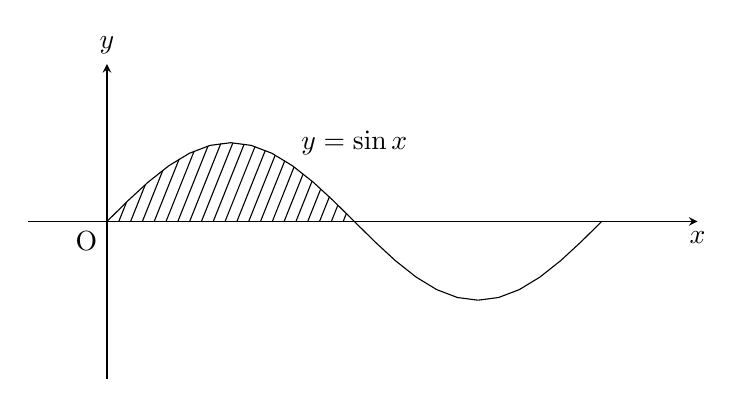
\begin{tikzpicture}
  \path[draw] plot[domain=0:2*pi] ({\x},{sin(\x r)});
  \path[draw,->,>=stealth] (0, -2) -- (0, 2) node[above]{$y$};
  \path[draw,->,>=stealth] (-1, 0) -- (7.5, 0) node[below]{$x$};
  \node at (pi,1) {$y=\sin x$};
  \node[below left] at (0,0){$\mathrm{O}$};
  \begin{scope}
    \path[clip] plot[domain=0:pi] ({\x}, {sin(\x r)}) -- cycle;
    \foreach \t in {1,2,...,20}{
      \path[draw] (0.15*\t, 0) -- (0.15*\t + 0.4, 1);
    }
  \end{scope}
\end{tikzpicture}


\begin{figure}[H]
  \centering
  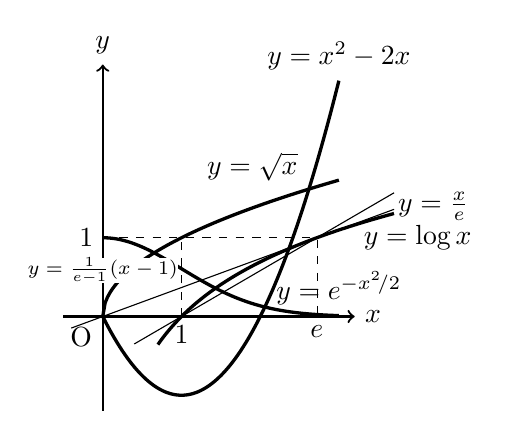
\begin{tikzpicture}[domain=0:3, samples=100, very thick] % 定義域、点の数、線幅
    \draw (0,0) node[below left]{O}; % 原点、0でも、above, below, left, rightで位置指定
    % 位置指定はanchor=north, south, east, westでも可能
    \draw[thick, ->] (-0.5,0)--(3.2,0) node[right] {$x$}; % x軸、[->]で矢印、他に[-stealth]等
    \draw[thick, ->] (0,-1.2)--(0,3.2) node[above] {$y$}; % y軸

    \draw plot(\x, {sqrt(\x)}) node at(1.9,1.9) {$y=\sqrt{x}$}; % atでnodeの位置指定
    \draw plot(\x, \x*\x-2*\x) node[above] {$y=x^2-2x$}; % 多項式
    \draw plot(\x, {exp(-0.5 * \x * \x)}) node[above] {$y=e^{-x^2\!/2}$}; % exp

    \draw [domain=0.7:3.7] plot(\x, {ln(\x)}); % y=log(x) 定義域を個別指定
    \node at(4,1) {$y=\log x$};

    \draw [thin, domain=-0.4:3.7] plot(\x,\x/e); % y=x/e、細線幅
    \node at(4.2,1.4){$y=\frac{x}{e}$};
    \draw [thin, domain=0.4:3.7] plot(\x, {(\x-1)/(e-1)});  % y=(x-1)/(e-1)
    \node [above, font=\scriptsize, fill=white, inner sep=0pt] % 途中で改行
    at(0,0.4){$y=\frac{1}{e-1}(x-1)$}; % node追加設定

    \draw [very thin, dashed](0,1) node [left]{$1$}--(e,1)--(e,0) node[below]{$e$}; % 補助線
    \draw [very thin, dashed](1,0) node [below]{$1$}--(1,1);
  \end{tikzpicture}
  \label{fig:tikz-3}
  \caption{tikzの例2}
\end{figure}


  

\end{document} % -------------------

